%************************************************
\chapter{Related Models}
\label{chapter:related_models}
%************************************************

\section{Reflection in Computer Science}

The term reflection is a commonly used word in computer science and
AI.  The idea is extremely simple and is a modelling contribution of
this thesis, but because of its simplicity, it is a widely applicable
idea.  In fact, \cite{maes:1988} distinguishes over 30 different types
of \emph{computational reflection}, grounded in the computer science
literature.  The type of computational reflection that is introduced
in this dissertation is not included in Maes' overview, although the
implementation of this model is based on many of the forms of
computational reflection that Maes does describe, e.g. procedural
reflection, type reflection, frame reflection, and others.  She does
not mention the type of reflection that I focus on in this thesis
because it was not at the time commonly considered computational.  The
type of reflection that is modelled here is a psychological type of
reflection: the ability to think about accomplishing thinking goals in
addition to thinking about accomplishing physical goals.  This
psychological form of reflection is modelled as two layers of control
in this thesis.  The first layer learns to control the physical world,
while the second layer learns to control the first layer.

\section{The Emotion Machine v1.0}

One previously developed cognitive architecture that implements
commonsense reasoning, based on Minsky's Emotion Machine theory of
mind \cite[]{minsky:2006}, is a metareasoning system for correcting
faulty plans, called EM-ONE (Emotion Machine, v1)
\cite[]{singh:2005b}. EM-ONE is written in Lisp, using a Prolog
extension as a logical resolution tool. EM-ONE is a layered
architecture consisting of reactive, deliberative, and reflective
layers. Mental critics are represented as commonsense narratives that
result in queries to a collection of different Prolog knowledge
bases. The commonsense narratives are given to the system in a Lisp
format that is compiled into the knowledge bases as collections of
horn clauses. These knowledge bases consist of collections of
domain-specific horn clauses that are divided into physical, social,
and mental domains of reasoning. On top of this Prolog logical
substrate, the Lisp program is organized into layers as a
critic-selector model of mind. The narrative plans that are generated
by the deliberative layer are executed by a lower-layer, called the
reactive layer. Part of the reactive layer of the algorithm is written
in C and runs PID control loops in a simulated social two-wheeled
inverted pendulum type robot. EM-ONE demonstrates how a system can use
commonsense narratives in order to reason by analogy in order to
generate plans. Also, EM-ONE demonstrates a learning process that is a
carefully crafted collection of reflective critics that recognize
types of social failures to infer the goals of other AIs.  Because of
the complexity of the rigid-body physics in the world, sometimes even
the most carefully constructed plans fail. EM-ONE has a layer of
reflective critics that debug deliberative narratives as they are
being interpreted by using a collection of commonsense narrative
debugging critics.  Using narratives about social situations, EM-ONE
infers the goals of the other AIs in the world given partial knowledge
of their visible physical actions. When mistakes are made in this
inference process, the failure is recognized reflectively, after the
fact. Specific types of debugging responses are implemented for
different forms of critical failures. EM-ONE is a step toward a large
and complex commonsense reasoning AI with multiple layers of
metareasoning that inspect, control, and debug mental representations.

In my AI, I have focused on implementing a form of learning where
resource executions are of constant time complexity, $O(1)$, so that
there are no search algorithms operating ``behind the scenes'', such
as those in any system based on Prolog with its implicit logical
resolution of declarative program statements.  The substrate presented
in this thesis is developed with the intention of building a stable
platform for larger cognitive architectures in the same vein as
EM-ONE.  For this reason, the substrate presented in this thesis is
distributed as an extensible open-source program that can be easily
downloaded, modified and used by others.  The rigid body physics
simulation implemented in EM-ONE has been extended in capability with
our kitchen cooking simulator, IsisWorld \cite[]{smith:2010}, which
allows experimenting with multiple social AIs in a rigid-body physical
kitchen that can work together to learn how to perform cooperative
cooking tasks.

\section{HACKER}

A good precedent for reflective debugging responses to catalogs of
failures is \emph{HACKER}, one of the first reflective planning and
debugging models, written by \cite{sussman:1973}.  [complete]

\section{EM-ONE}

\cite{singh:2005b} provided \emph{EM-ONE}, a most recent example of an
extension of HACKER that reasons about a more complicated
three-dimensional physical and social block building domain.
[complete]

\section{Propagators}

\cite{radul_and_sussman:2009} describe an object called a \emph{cell}
that is closely related to the knowledge dependencies depicted in
{\mbox{\autoref{figure:dependency_traces}}}.  These cells can be
connected by dependency sets that specify functions that derive new
knowledge from the dependencies, as well as, functions for merging the
collected knowledge in cells.  Collections of Radul and Sussman's
cells are called a \emph{propagator}.  The knowledge dependencies in
this model can be thought of as a type of propagator.  The combination
of a propagator model of knowledge maintenance with a reflective
organization is described as future research in
\autoref{chapter:future}.
%\begin{figure}
%\center
%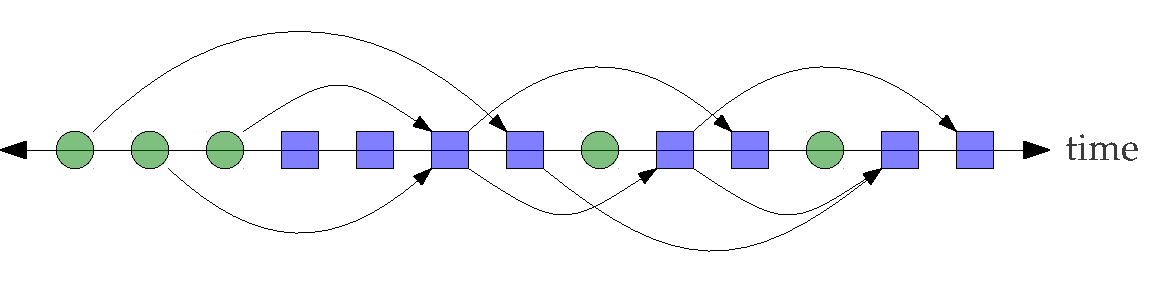
\includegraphics[width=10cm]{gfx/dependency_traces}
%\caption{Dependency traces as propagator cells.}
%\label{figure:propogators_dependency_traces}
%\end{figure}

\section{Interior Grounding}

\cite{minsky:2005} describes an evolutionary reflective model of mind
called \emph{interior grounding}.  Interior grounding states that each
layer of reflective thinking could be genetically predestined to each
have different and specific types of useful ways of thinking.  Minsky
rejects the \emph{physical grounding hypothesis}, which stipulates
that thoughts must necessarily develop from the lowest layer first and
only subsequently to the higher layers of thinking.

Because my AI is modelled after Minsky's Emotion Machine cognitive
architecture, activities in the mind can create and manipulate
symbolic arrangements without these symbols necessarily referring to
the physical layer of activity.  My model considers factual grounding
in both the perception of physical knowledge as well as the perception
of internal mental states, such as the deliberative planning machine
knowledge.

In terms of the Emotion Machine cognitive architecture, each
reflective layer of my model can be considered to have a unique
built-in reactive layer, which makes room for these genetic
dispositions that Minsky describes as the basis for interior
grounding.  My AI demonstrates interior grounding by having sets of
factual knowledge as the control domain for both the deliberative as
well as the reflective planning machines, so factual grounding of
hypothetical counterfactual inferences in my AI need not begin by
reasoning about physical activity, growing from lower layers to higher
layers, but may instead begin by reasoning about the factual events in
the deliberative planning machine knowledge bases.

\section{Metareasoning}

\cite{cox_and_raja:2008,cox:2010} present a reflective model of mind
called \emph{metareasoning}.  My AI demonstrates metareasoning in the
reflective layer, which controls the deliberative planning machine.
The metareasoning described by Cox and Raja begins with a ``ground
level'', which corresponds to the physical knowledge base in my AI,
then describe how a second level, the ``object level'', is a control
loop that receives perceptions from the ground level, processes these,
and sends actionable commands back to the ground level.  The
metacognitive object level corresponds with the deliberative layer and
the deliberative planning machine knowledge base in my AI.  They then
proceed to a third level, which completes two cascaded control loops:
one controlling the ground level with another controlling the object
level.  This third level is called the ``meta-level''.  Cox and Raja's
meta-level corresponds to the reflective layer and reflective planning
machine knowledge base in my AI.
\begin{figure}[bth]
\begin{align*}
\text{Cox and Raja's Ground Level } &{\approx} \text{ Reactive Layers} \\
\text{Cox and Raja's Object Level } &{\approx} \text{ Deliberative Layer} \\
\text{Cox and Raja's Meta-Level }   &{\approx} \text{ Reflective Layer}
\end{align*}
\caption{The lower levels of Cox and Raja's metareasoning model mapped
  to the Emotion Machine cognitive architecture presented in this
  thesis.}
\label{figure:metareasoning_as_reflective_order_notation}
\end{figure}
\autoref{figure:metareasoning_as_reflective_order_notation} shows how
Cox and Raja's levels map to the Emotion Machine cognitive
architecture presented in this thesis.  Here they explain what happens
when the object level fails in either the creation or execution of a
plan:
\begin{quote}
When reasoning fails at some task, it may involve the explanation of
the causal contributions of failure and the diagnosis of the
object-level reasoning process.
\end{quote}
Cox and Raja explain how debugging causal models of the reasoning
process itself is a form of meta-level reasoning, or reflective layer
of thinking.  My model has a separate distinct class of resource
activation hypotheses for the separate layers of deliberative and
reflective thinking, so learning physical causal models is a distinct
activity from reflectively learning deliberative thinking causal
models.  The implementation demonstrates how two distinct layers of
hypothetical inference models allow not only learning to act but also
learning to think about acting.

